%%%%%%%%%%%%%%%%%%%%%%%%%%%%%%%%%%%%%%%%%%%%%%%%%%%%%%%%%%%%%%%%%%%%%%%%
%
%		Chapter 3 - System Models
%
%%%%%%%%%%%%%%%%%%%%%%%%%%%%%%%%%%%%%%%%%%%%%%%%%%%%%%%%%%%%%%%%%%%%%%%%


\begin{topic}[Models of Systems]



\vfil

\begin{center}
\begin{minipage}{300pt}
	\includegraphics*[width=300pt]{images/chap3-xkcd.png}

	\hfill {\footnotesize (image from \href{https://www.xkcd.com/2063/}{xkcd - comic \#2063})}
\end{minipage}
\end{center}


\end{topic}






%%%%%%%%%%%%%%%%%%%%%%%%%%%%%%
%
%  MODULE - Modelling Two Interconnected Quantities
%
%%%%%%%%%%%%%%%%%%%%%%%%%%%%%%



\begin{module}{Modelling Two Quantities}
	\label{sys:model}

	In this module you will learn
\begin{itemize}
	\item how to model two or more inter-dependent quantities using systems
\end{itemize}

\hfill \\


Often, when modelling something, we are faced with two or more quantities that depend on each other. This means that one equation is not enough, so we need to learn how to deal with a system of equations. \\


Just like we did in module \ref{model-odes}, we will follow the step by step procedure developed in chapter 1.

\paragraph{\emph{Step 1.}} Define the problem

\begin{example}
We want to model two interacting populations, like the populations of bears and salmon in a specific natural park.\\

The first step is to decide on what we want to find at the end of the process. 
In this case, we want to know the number of individuals in each population and how they change as time passes. So we define:
\begin{itemize}
	\item $b(t) =$ number of bears in the natural park at time $t$;
	\item $s(t) =$ number of salmon in the natural park at time $t$.
\end{itemize}
\end{example}


\paragraph{\emph{Step 2.}} Build a mind map

\begin{example}
We start with both species in the centre:

\def\SalmonBear{
	\fill[color=orange!50!white] (-4,0) rectangle (-2,1) node[pos=.5] {\color{black}Salmon};
	\fill[color=brown!60!white] (4,0) rectangle (2,1) node[pos=.5] {\color{black}Bear};
}
\begin{center}
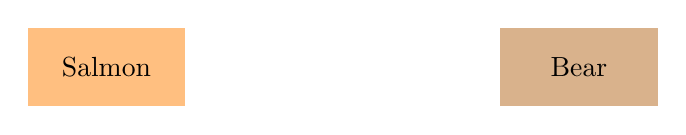
\begin{tikzpicture}
	\SalmonBear
\end{tikzpicture}
\end{center}

We can start brainstorming about the things that affect these populations:
\begin{center}
%\begin{tikzpicture}
%	\SalmonBear
%    \begin{scope}[decoration={
%    markings,
%    mark=at position 0.5 with {\arrow{>}}}
%    ]
%	\draw[postaction={decorate}] (-2,1) arc (120:60:4) node[pos=0.5,above] {food};
%    \draw[postaction={decorate}] (2,0) arc (300:240:4) node[pos=0.5,below] {hunts};
%    \end{scope}
%    \draw (-3,0) -- (-4,-1);
%    \fill[color=green!50!white] (-5.25,-2) rectangle (-2.75,-1) node[pos=.5] {\color{black}reproduction};
%    \draw (-3,1) -- (-4,2);
%    \fill[color=yellow!50!white] (-5.25,2) rectangle (-2.75,3) node[pos=.5] {\color{black}habitat limits};
%    \draw (3,0) -- (4,-1);
%    \fill[color=red!50!white] (5.25,-2) rectangle (2.75,-1) node[pos=.5] {\color{black}competition};
%    \draw (3,1) -- (4,2);
%    \fill[color=yellow!50!white] (5.25,2) rectangle (2.75,3) node[pos=.5] {\color{black}habitat limits};
%\end{tikzpicture}
\begin{tikzpicture}
	\SalmonBear
    \begin{scope}[decoration={
    markings,
    mark=at position 0.5 with {\arrow{>}}}
    ]
    \draw[postaction={decorate}] (-2,0.5) -- (2,0.5) node[pos=0.5,above] {food};
    \draw[postaction={decorate}] (2,0) arc (300:240:4) node[pos=0.5,below] {hunts};
    \end{scope}
    \draw (-3,0) -- (-4,-1);
    \fill[color=green!50!white] (-5.25,-2) rectangle (-2.75,-1) node[pos=.5] {\color{black}reproduction};
    \draw (-3,1) -- (-0.5,2);
    \draw (3,1) -- (0.5,2);
    \fill[color=yellow!50!white] (-1.5,2) rectangle (1.5,3) node[pos=.5] {\color{black}habitat limits};
    \draw (3,0) -- (4,-1);
    \fill[color=red!50!white] (5.25,-2) rectangle (2.75,-1) node[pos=.5] {\color{black}competition};
\end{tikzpicture}
\end{center}
	
\end{example}


\paragraph{\emph{Step 3.}} Make assumptions

\begin{example}
In this step, we discuss which of the boxes in the mind map we want to actually consider in our model, and which assumptions we need to make to consider them. \\

Let us start with how these species interact with each other:
\begin{enumerate}
	\item Salmon provide food for bears: the bear population profits from each encounter with salmon. How does each bear-salmon encounter affect the bear population?
	\item Bears hunt salmon: the salmon population is likely to decrease with each encounter with a bear. How does each bear-salmon encounter affect the salmon population?
\end{enumerate}

These two components are essential in our model, so we need to include them. It still leaves some freedom on how to do this. \\

There are other elements that we might want to include in our model:
\begin{enumerate}[start=3]
	\item Salmon reproduction: in the absence of predators and under ideal conditions, salmon should grow according to the Malthusian model, i.e. the rate of growth is proportional to the number of salmon;
	\item Bear competition: bears are mainly predators, so without salmon, their numbers will decrease, also according to the Malthusian model;
	\item Habitat limits: these species live in habitats that have limited resources, so we can consider a carrying capacity for each species.
\end{enumerate}

To make the model simpler, we will \emph{ignore habitat limits}. This means that this model will not be accurate if the populations become very large.
	
\end{example}


\paragraph{\emph{Step 4.}} Construct a model

\begin{example}
We will start with our populations:
\begin{itemize}
	\item $b(t)$
	\item $s(t)$
\end{itemize}
and we will start adding components to each of these one by one. \\

For the first two items, we need to estimate the number of encounters salmon-bear. We assume that the number of encounters is proportional to the number of all possible encounters: $b(t) s(t)$.

\begin{enumerate}
	\item Salmon provide food for bears: 
\end{enumerate}

\end{example}


	\begin{exercises}

	\begin{problist}
	
	\prob Create a model for two cooperating populations, like sharks and remoras. 
	
	
%	\begin{center}
%		\includegraphics*[height=150pt]{images/module15-spring-mass-dashpot.pdf}
%	\end{center}
	
	
	\begin{minipage}{.35\textwidth}
		\prob We have a spring attached to a mass and with a dashpot. 
		\begin{enumerate}
			\item Model the position of the mass as time changes.
			\item Obtain a system of two first-order ODEs. Remember to explain how the new functions relate to the spring-mass-dashpot system.
		\end{enumerate}
	\end{minipage}
	\hfill
	\begin{minipage}{100pt}
		\includegraphics*[height=100pt]{images/module15-spring-mass-dashpot.pdf}
	\end{minipage}

	\prob Model a vehicle with a special engine that provides an acceleration to the car proportional to the fuel left.
	
	\prob Imagine two twin babies and model their crying volume. Assume that they naturally become tired and stop crying if alone, but they cry more if the other twin is crying.
	
	
	
	\begin{minipage}{.35\textwidth}
		\prob Create a simplified model for a tree, considering the height of the tree and its leaf area and how they affect each other.	
	\end{minipage}
	\hfill
	\begin{minipage}{100pt}
		\includegraphics*[height=100pt]{images/module15-tree.pdf}
	\end{minipage}

	\prob Create a model on how a student's confidence in her own ability affects her learning/knowledge of a subject. Remember the Ebbinghaus' ``forgetting curve''.

	\begin{center}
		\includegraphics*[width=125pt]{images/module15-UofT2YYZ.pdf}	
	\end{center}

	\prob Imagine that there are two ways to travel from UofT to Toronto's Pearson airport (YYZ). Both paths take the same time if there is no traffic. You want to direct people on the fastest path. Create a model for choosing the fastest path.
	
	
	\prob Create a model for the sales of a specific brand of sneakers. The goal is to capture the influence of famous people and non-famous people on each other's purchases.
	
	\prob Create a model on how the population and the cost of living in Toronto affect each other.
	
	
	\end{problist}
\end{exercises}

\end{module}



\begin{lesson}
	\Title{Modelling Two Quantities}

	\Heading{Objectives}
	\begin{itemize}
		\item Bla
	\end{itemize}
	
	\Heading{Motivation} 

\end{lesson}




\newpage

\question
	Core Exercise with several parts
\begin{parts}
	\item Part 1
	\item Part 2
\end{parts}

\bookonlynewpage


\question
	One more core exercise




%%%%%%%%%%%%%%%%%%%%%%%%%%%%%%
%
%  MODULE - Solving Systems
%
%%%%%%%%%%%%%%%%%%%%%%%%%%%%%%



\begin{module}{Systems of two linear ODEs with constant coefficients}
	\label{sys:solve}

	In this module you will learn
\begin{itemize}
	\item how to solve systems of two linear first-order ODEs with constant coefficients
\end{itemize}

\hfill \\


First, a system of two first-order ODEs has the form:
$$
\begin{cases}
x'(t) = f\big(t, x(t),y(t)\big) \\	
y'(t) = g\big(t, x(t),y(t)\big)
\end{cases}
$$
where the functions $f$ and $g$ are continuous and have continuous derivatives. \\

This system could be nonlinear, so we are only considering linear systems with constant coefficients, which means that they have a very specific form:
$$
\begin{cases}
	x'(t) = a x(t) + b y(t) + e\\
	y'(t) = c x(t) + d y(t) + f
\end{cases}
%
\quad \Leftrightarrow \quad 
	\begin{bmatrix} x'(t) \\ y'(t) \end{bmatrix}
	=
	\begin{bmatrix} a & b \\ c & d \end{bmatrix}
	\begin{bmatrix} x(t) \\ y(t) \end{bmatrix}
	+	\begin{bmatrix} e \\ f \end{bmatrix}
%
\quad \Leftrightarrow \quad 
	\vec{r}'(t)
	=
	A \, \vec{r}(t) + \vec{b}
$$
where
$$
\vec{r}(t) = \begin{bmatrix} x(t) \\ y(t) \end{bmatrix}
\quad , \quad 
A = \begin{bmatrix} a & b \\ c & d \end{bmatrix}
\quad and \quad 
\vec{b}=\begin{bmatrix} e \\ f \end{bmatrix}.
$$

The unknown functions we are trying to find is $\vec{r}(t)$. \\


\paragraph{\emph{Homogeneous Systems.}} These are systems of the form above with $\vec{b} = \vec{0}$.

This means that we want to find all functions $\vec{r}(t)$ that satisfy
$$
\vec{r}'(t) = A \vec{r}(t).
$$


\begin{example}
Let us start with an example of the same problem where $\vec{r}(t)$ is a ``one-dimensional'' vector, a scalar function $u(t)$, and the matrix $A$ is a ``one-dimensional matrix'', a constant $a$. \\

We want to solve the problem	
$$
u'(t) = a \cdot u(t).
$$

We have seen how to solve these kind of problems before. The solutions are
$$
u(t) = c e^{at},
$$
where $c$ can be any constant.
\end{example}

In our two-dimensional case, it is a little more complicated. We can't just write $e^{At}$ where $A$ is a matrix (this expression can make sense, but we would have to find out what is the exponential of a matrix). \\

So we can use the example above to make an \emph{educated guess}: the solution should look like an exponential:
$$
\vec{r}(t) = 
\vec{c} \, e^{\lambda t},
$$
where $\vec{c}$ is a constant vector. \\

If our guess is correct, to find $\vec{r}(t)$, we only need to find $\lambda$ and $\vec{c}$. \\

Let us see what happens when we use this guess and plug it into the system of ODEs:
\begin{align*}
\vec{r}'(t) = A \vec{r}(t) \quad
	& \Leftrightarrow \quad \vec{c} \lambda e^{\lambda t} = A \vec{c} e^{\lambda t} \\
	& \Leftrightarrow \quad \vec{c} \lambda = A \vec{c}.
\end{align*}

This is a problem you have seen before -- and eigenvalue-eigenvector problem: 
\begin{itemize}
	\item $\lambda$ can be any eigenvalue of the matrix $A$
	\item $\vec{c}$ can be any eigenvector of $A$ associated with $\lambda$ 
\end{itemize}

This means that we might have multiple choices for eigenvalues and eigenvectors, or even that eigenvalues and eigenvectors involve complex numbers.
Let us split our study of possible solutions in three cases.



%%%%%%%%%       %%%%%%%%%       %%%%%%%%%       %%%%%%%%%       %%%%%%%%%

\subsection{Two real and distinct eigenvalues}

\begin{example}
Consider the problem
$$
\vec{r}'(t) = \begin{bmatrix}	
 10 & 18 \\ -6 & -11	
 \end{bmatrix} \, \vec{r}(t).
$$

Then, the eigenvalues and eigenvectors of the matrix are
\begin{itemize}
	\item $\lambda_1=-2$ with eigenvector $\vec{v}_1 = \begin{bmatrix} 3 \\ -2 \end{bmatrix}$
	\item $\lambda_2=1$ with eigenvector $\vec{v}_2 = \begin{bmatrix} 2 \\ -1 \end{bmatrix}$
\end{itemize}

This means that we found two solutions:
$$
\vec{r}_1(t) = \begin{bmatrix} 3 \\ -2 \end{bmatrix} e^{-2t}
\quad \text{ and } \quad \vec{r_2}(t) = \begin{bmatrix} 2 \\ -1 \end{bmatrix} e^{t}.
$$

Then, we can show that 
$$
\vec{r}(t) = c_1 \begin{bmatrix} 3 \\ -2 \end{bmatrix} e^{-2t}
+c_2\begin{bmatrix} 2 \\ -1 \end{bmatrix} e^{t}
$$
is also a solution of the problem for any constants $c_1$ and $c_2$.

In fact, we can show that this formula captures all possible solutions for this problem.
\end{example}


\begin{video}
	\begin{itemize}
		\item \qrvideo{https://youtu.be/YUjdyKhWt6E}
	\end{itemize}
\end{video}




%%%%%%%%%       %%%%%%%%%       %%%%%%%%%       %%%%%%%%%       %%%%%%%%%

\subsection{Two complex eigenvalues}

We actually don't need to know a lot about complex numbers to be able to understand how to solve this case.
The results about complex values that are necessary to know will be included in the box below.

\begin{definition}[Complex numbers]
\begin{itemize}
	\item A complex number is a number of the form $z=a+ib$ where $i$ is called the imaginary constant and satisfies $i^2=-1$.
	\item Given a complex number $z=a+ib$, we call $\overline{z}=a-ib$ its complex conjugate. It satisfies:
	$$ z \cdot \overline{z} = a^2+b^2 = |z|^2.$$

	\item If a matrix has real components and two complex eigenvalues, then the eigenvalues are complex conjugates of each other. Moreover, the eigenvectors are also complex conjugates of each other.
	\item Euler's Formula: $e^{i \theta} = \cos(\theta) + i \sin (\theta)$.
\end{itemize}
\end{definition}




\begin{example}
Consider the problem
$$
\vec{r}'(t) = \begin{bmatrix}	
 1 & 1 \\ -1 & 1
 \end{bmatrix} \, \vec{r}(t).
$$

Then, the eigenvalues and eigenvectors of the matrix are
\begin{itemize}
	\item $\lambda_1=1+i$ with eigenvector $\vec{v}_1 = \begin{bmatrix} -i \\ 1 \end{bmatrix}$
	\item $\lambda_2=1-i$ with eigenvector $\vec{v}_2 = \begin{bmatrix} i \\ 1 \end{bmatrix}$
\end{itemize}

This means that we found two solutions:
$$
\vec{r}_1(t) = \begin{bmatrix} -i \\ 1 \end{bmatrix} e^{(1+i)t}
\quad \text{ and } \quad \vec{r}_2(t) = \begin{bmatrix} i \\ 1 \end{bmatrix} e^{(1-i)t}.
$$

Then, all solutions of this system of ODEs can be expressed as
$$
\vec{r}(t) = c_1 \begin{bmatrix} -i \\ 1 \end{bmatrix} e^{(1+i)t}
+c_2\begin{bmatrix} i \\ 1 \end{bmatrix} e^{(1-i)t}.
$$

There is a problem with the form of these solutions: they involve complex numbers!

Imagine that we start with a problem where we have two (real) quantities that interact with each other through this system of differential equations.
Then we expect these quantities to measure in real numbers, not complex.

\begin{itemize}
	\item This means that we expect \emph{the imaginary part of this solutions to cancel out}.
\end{itemize}

So let us manipulate this formula using Euler's formula and see if we can re-write in such a way that doesn't involve complex numbers. \\

We have:
\begin{align*}
	e^{(1+i)t} &= e^t \cdot e^{it} = e^t \big( \cos(t) + i \sin(t)\big) \\
	e^{(1-i)t} &= e^t \cdot e^{-it} = e^t \big( \cos(t) - i \sin(t)\big)
\end{align*}

So our solution expands to:
$$
\vec{r}(t) = c_1 \begin{bmatrix} -i \\ 1 \end{bmatrix} e^t \big( \cos(t) + i \sin(t)\big)
+c_2\begin{bmatrix} i \\ 1 \end{bmatrix} e^t \big( \cos(t) - i \sin(t)\big).
$$

We can now manipulate this expression:
\begin{align*}
\vec{r}(t) 
	& = e^t
		\begin{bmatrix}
			-i c_1 	\big( \cos(t) + i \sin(t)\big) + i c_2 \big( \cos(t) - i \sin(t)\big) \\
			c_1 	\big( \cos(t) + i \sin(t)\big) + c_2 \big( \cos(t) - i \sin(t)\big) \\
		\end{bmatrix} \\
	& = e^t 
		\begin{bmatrix}
			(c_1+c_2) \sin(t) - i (c_1-c_2) \cos(t) \\
			(c_1+c_2) \cos(t) + i(c_1-c_2) \sin(t)
		\end{bmatrix} \\
	& = e^t \left( (c_1+c_2) \begin{bmatrix} \sin(t) \\ \cos(t) \end{bmatrix}
		+ i (c_1 -c_2) \begin{bmatrix} - \cos(t) \\ \sin(t) \end{bmatrix}
		\right)
\end{align*}

So now we do something that might look like a ``cheating''. We define:
$$
a_1 = c_1+c_2 \quad \text{ and } \quad a_2 = i (c_1-c_2).
$$


Then the solution is
$$
\vec{r}(t) = a_1\begin{bmatrix} \sin(t) \\ \cos(t) \end{bmatrix} e^t
		+ a_2 \begin{bmatrix} - \cos(t) \\ \sin(t) \end{bmatrix} e^t.
$$

This last form doesn't include any complex numbers and is equivalent to the previous form.

\end{example}

\begin{graybox}
	It may look like the final solution above still includes complex numbers in the constants $a_1$ and $a_2$. 
	
	To convince yourself that this is not the case, solve the following exercise.\\
	
	Find the unique solution of
	$$
	\vec{r}'(t) = \begin{bmatrix}	
 		1 & 1 \\ -1 & 1
		\end{bmatrix} 
		\, \vec{r}(t)
	\qquad \text{ with} \qquad
	\vec{r}(0) = \begin{bmatrix}
 			-3 \\ 2
	 \end{bmatrix}
	 $$
	 
	 Find the constants $c_1, c_2$ and then the constants $a_1,a_2$. Which ones are complex and which ones are real?
\end{graybox}

\begin{video}
	\begin{itemize}
		\item \qrvideo{https://youtu.be/TRVS5Wo9LoM}
	\end{itemize}
\end{video}



%%%%%%%%%       %%%%%%%%%       %%%%%%%%%       %%%%%%%%%       %%%%%%%%%

\subsection{One real repeated eigenvalue}


\begin{example}
Consider the problem
$$
\vec{r}'(t) = \begin{bmatrix}	
 5 & 0 \\ 1 & 5	
 \end{bmatrix} \, \vec{r}(t).
$$

Then, there is only one eigenvalue with one eigenvector
\begin{itemize}
	\item $\lambda_1=5$ with eigenvector $\vec{v}_1 = \begin{bmatrix} 0 \\ 1 \end{bmatrix}$, which yield a solution $\vec{r}_1(t) = c_1 \begin{bmatrix} 0 \\ 1 \end{bmatrix} e^{5t}$.
\end{itemize}

This is a \emph{problem} because we need two solutions to put together and obtain two constants, as in the two previous cases.
%\end{example}

\begin{graybox}
To convince yourself that it is a problem, try solving the problem above with initial conditions
$$
\vec{r}(0) = \begin{bmatrix}	0 \\ 4 \end{bmatrix}.
$$

What about with initial conditions
$$
\vec{r}(0) = \begin{bmatrix}	 1 \\ 4 \end{bmatrix} \quad ?
$$
\end{graybox}

%\begin{example}

This means that we ware missing one solution -- that will enable us to solve the problem for any initial conditions. \\


Let us re-write the original problem in a different form by letting 
$$
\vec{r}(t) = \begin{bmatrix} x(t) \\ y(t)\end{bmatrix}.
$$
Then we have
$$
\begin{cases}
x'(t) = 5 x(t) \\
y'(t) = x(t) +5 y(t)	
\end{cases}
$$
These are two ODEs, but we can solve the first and then tackle the second one.
We obtain
$$
\begin{cases}
	x(t) = c_2 e^{5t} \\
	y(t) = 	c_1 e^{5t} + c_2 t e^{5t} 
\end{cases}
\quad \Leftrightarrow \quad
	\vec{r}(t) = \begin{bmatrix}
		c_2 \\ c_1 + c_2 t
	\end{bmatrix} e^{5t}
\quad \Leftrightarrow \quad
	\vec{r}(t) = c_1 \begin{bmatrix} 0 \\ 1 \end{bmatrix} e^{5t} + c_2
	\begin{bmatrix}	1 \\ t
	\end{bmatrix} e^{5t}
$$
\end{example}

\begin{graybox}
Observe that the solution we found has the form:
$$
	\vec{r}(t) = \underbrace{c_1 \begin{bmatrix} 0 \\ 1 \end{bmatrix} e^{5t}}_{\text{solution } \vec{r}_1(t)} + c_2 \left( 
	\underbrace{\begin{bmatrix}	1 \\ 0 \end{bmatrix}}_{\text{new vector } \vec{w}} e^{5t} + \underbrace{\begin{bmatrix} 0  \\ 1 
	\end{bmatrix}}_{\vec{v}_1} t e^{5t}\right).
$$

So we can make another \emph{educated guess} that the solution we were missing has the form:
$$
\vec{r}_2(t) = \left(\vec{w} + \vec{v}_1 t\right) e^{\lambda t}.
$$

With this form in mind, we can plug it into the system of ODEs \quad $\vec{r}'(t) = A \vec{r}(t)$ \quad, which has exactly one eigenvalue $\lambda$, to get:
$$
\lambda \vec{w}e^{\lambda t} + \lambda \vec{v}_1 t e^{\lambda t} + \vec{v}_1 e^{\lambda t}
= A \vec{w} e^{\lambda t} + A \vec{v}_1 t  e^{\lambda t}
$$
which is equivalent to:
$$
\lambda \vec{w} + \underbrace{\lambda \vec{v}_1}_{=A \vec{v}_1} t  + \vec{v}_1
= A \vec{w}  + A \vec{v}_1 t 
	\quad \Leftrightarrow \quad
	\left( \lambda I - A \right ) \vec{w} = \vec{v}_1
$$
%which becomes
%$$
%\lambda \vec{w} + \vec{v}_1
%= A \vec{w}  
%	\quad \Leftrightarrow \quad
%	\left( \lambda I - A \right ) \vec{w} = \vec{v}_1
%$$

Since at this point we already know $\lambda$ and $\vec{v}_1$, we can now find $\vec{w}$ in a similar way used to find the eigenvector $\vec{v}_1$. The vector $\vec{w}$ is called a \emph{generalized eigenvector} of $A$ associated with the eigenvalue $\lambda$.

\end{graybox}

\begin{video}
	\begin{itemize}
		\item \qrvideo{https://youtu.be/hCShTLmeZN4}
	\end{itemize}
\end{video}






	\begin{exercises}

	\begin{problist}
	\prob Find the general solution of the problem $\vec{r}'(t) = A \vec{r}(t)$ for the following matrices:
	\begin{enumerate}
	\begin{minipage}{.2\textwidth}
		\item $A = \begin{bmatrix} -7 & 6 \\ -9 & 8 \end{bmatrix}$;
		\item $A = \begin{bmatrix} 22 & 24 \\ -15 & -16\end{bmatrix}$;
		\item $A = \begin{bmatrix} 0 & 1 \\ -5 & 0 \end{bmatrix}$;
		\item $A = \begin{bmatrix} 0 & 1 \\ 5 & 0 \end{bmatrix}$;
		\item $A = \begin{bmatrix} 1 & \sqrt{3} \\ \sqrt{3} & -1\end{bmatrix}$;
		\item $A = \begin{bmatrix} 1 & \sqrt{3} \\ -\sqrt{3} & 1\end{bmatrix}$;
	\end{minipage}
	\qquad
	\begin{minipage}{.2\textwidth}
		\item $A = \begin{bmatrix} 0 & 1 \\ -4 & -4 \end{bmatrix}$;
		\item $A = \begin{bmatrix} -4 & -6 \\ 2 & 3 \end{bmatrix}$;
		\item $A = \begin{bmatrix} 2 & -3 \\ 0 & 2 \end{bmatrix}$;
		\item $A = \begin{bmatrix} 2 & 0 \\ 0 & 2 \end{bmatrix}$;
		\item $A = \begin{bmatrix} 0 & 0 \\ 1 & 0\end{bmatrix}$; 
		\item $A = \begin{bmatrix} 0 & 0 \\ 0 & 1\end{bmatrix}$; 
	\end{minipage}
	\end{enumerate}

	\prob For each of the problems in the previous exercise, find the solution that satisfies the initial conditions:
	\begin{enumerate}[label=(\roman*)]
		\item $\vec{r}(0)=\begin{bmatrix} 0 \\ 0 \end{bmatrix}$;
		\item $\vec{r}(0)=\begin{bmatrix} 1 \\ 3 \end{bmatrix}$;
		\item $\vec{r}(1)=\begin{bmatrix} -2 \\ 2 \end{bmatrix}$.
	\end{enumerate}


	\prob Consider the problem $\vec{r}'(t) = \begin{bmatrix} 2 & 0 \\ 1 & 3 \end{bmatrix} \vec{r}(t) + \begin{bmatrix} -2 \\ 11 \end{bmatrix}$.
	\begin{enumerate}
		\item Show that $\vec{e}(t) = \begin{bmatrix} 1 \\ -4 	\end{bmatrix}$ is a solution of this problem.
		\item Find the general solution of 
		$$\vec{u}'(t) = \begin{bmatrix} 2 & 0 \\ 1 & 3 \end{bmatrix} \vec{u}(t).$$
		\item Let $\vec{r}(t) = \vec{u}(t) + \vec{e}(t)$. Show that this is a solution of the original problem.
		\item Let $\vec{r}_1(t)$ and $\vec{r}_2(t)$ be two solutions of the original problem. 
		\begin{enumerate}
			\item Is $\vec{r}_1(t) + \vec{r_2}(t)$ a solution? 
			\item Is $3\vec{r}_1(t) $ a solution? 
			\item Write a result on how one can safely combine solutions of non-homogeneous problems.
		\end{enumerate}
	\end{enumerate}

	
	\prob \label{prob:sys-nonhomogeneous}Consider the problem  \quad $\vec{r}'(t) = \begin{bmatrix} 1 & 2 \\ 3 & 0 \end{bmatrix}
 \vec{r}(t)+\begin{bmatrix} -5 \\ 3 \end{bmatrix}
$.
	\begin{enumerate}
		\item Observe that this system is an autonomous system of ODEs. What is the equilibrium solution? 
		\item Let the equilibrium solution solution you just found be called $\vec{e}$. Consider $\vec{u}(t) = \vec{r}(t) - \vec{e}$, where $\vec{r}(t)$ is the solution of the original problem. Show that 
			$$ \vec{u}'(t) = A \, \vec{u}(t).$$
		\item Find $\vec{u}(t)$.
		\item Find $\vec{r}(t)$.
		\item Write a procedure to solve any problem of the form
			$$ \vec{r}(t) = A \, \vec{r}(t) + \vec{b}. $$
	\end{enumerate}
	
	
	\prob \label{prob:sys-superposition}Consider the problem \quad $\vec{r}'(t) = A \, \vec{r}(t)$.
	Assume that we have two solutions $\vec{r_1}(t)$ and $\vec{r_2}(t)$.
	\begin{enumerate}
		\item Show that $\vec{r}(t) = \vec{r_1}(t) + \vec{r_2}(t)$ is a solution also.
		\item Show that $\vec{r}(t) = 2\vec{r_1}(t) - 3\vec{r_2}(t)$ is a solution also.
		\item Find all possible solutions of the problem.
	\end{enumerate}
	
	
		\prob Consider the problem $\vec{r}'(t) = \begin{bmatrix} 1 & -2 \\ -2 & 1 \end{bmatrix} \vec{r}(t)$.
		\begin{enumerate}
			\item Find the solution that satisfies the initial condition $\vec{r}(0)=\begin{bmatrix}1 \\ 0\end{bmatrix}$. Call it $\vec{u}(t)$.
			\item Find the solution that satisfies the initial condition $\vec{r}(0)=\begin{bmatrix}0 \\ 1\end{bmatrix}$. Call it $\vec{v}(t)$.
			\item Define the matrix function
			$$ \Phi(t) = \begin{bmatrix} \vec{u}(t) \; | \; \vec{v}(t) \end{bmatrix} = \begin{bmatrix} u_1(t) & v_1(t) \\ u_2(t) & v_2(t) \end{bmatrix}.$$
			
			Show that $\vec{r}(t) = \Phi(t) \vec{r}_0$ is a solution of the original system of ODEs. Which initial condition does it satisfy?
			
			\item Write a result relating $\Phi(t)$ to the solution of initial-value problems.
			\end{enumerate}

	
	
		\prob \label{mod16:prob-W1}Consider a system of ODEs $\vec{r}'(t) = A \vec{r}(t)$ with two solutions $\vec{r}_1(t)$ and $\vec{r}_2(t)$. 
		
		We want to study the conditions that are necessary on the solutions $\vec{r}_1$ and $\vec{r}_2$ to guarantee that we can solve any initial-value problem.
		
		\begin{enumerate}
			\item What is the general solution for this problem?
			\item If the initial condition is $\vec{r}(0)= \begin{bmatrix} 1 \\ 2 \end{bmatrix}$, then what are the conditions on $\vec{r}_1,\vec{r}_2$ ?
			\item If the initial condition is $\vec{r}(0)= \vec{r_0}$, then what are the conditions on $\vec{r}_1,\vec{r}_2$ ?
		\end{enumerate}

		\prob Consider a system of ODEs $\vec{r}'(t) = A \vec{r}(t)$ with two solutions $\vec{r}_1(t), \vec{r}_2(t)$.
		
			Let $R(t)$ be the matrix 
				$R(t) = \begin{bmatrix} \vec{r}_1(t) & | & \vec{r}_2(t)	\end{bmatrix} $ 
				and let $W(t) = \det R(t)$.
		
		\begin{enumerate}
			\item Show that $W(t)$ is a solution of $W' = (a_{11} + a_{22}) W$.
			\item Solve the ODE above to obtain an expression for $W(t)$.
			\item Show that $W(t)$ is either identically zero, or it's never zero. 
			\item Use this result to simplify your answer to problem \ref{mod16:prob-W1}(c).
		\end{enumerate}
	
	\end{problist}
\end{exercises}

\end{module}



\begin{lesson}
	\Title{Systems of two linear ODEs with constant coefficients}

	\Heading{Objectives}
	\begin{itemize}
		\item Bla
	\end{itemize}
	
	\Heading{Motivation} 

\end{lesson}




\newpage

\question
	Core Exercise with several parts
\begin{parts}
	\item Part 1
	\item Part 2
\end{parts}


\bookonlynewpage


\question
	One more core exercise




%%%%%%%%%%%%%%%%%%%%%%%%%%%%%%
%
%  MODULE - Phase Portraits
%
%%%%%%%%%%%%%%%%%%%%%%%%%%%%%%



\begin{module}{Phase Portraits}
	\label{sys:phase}

	In this module you will learn
\begin{itemize}
	\item what is an autonomous differential equation
	\item how to obtain some properties of solutions of autonomous differential equations without solving them
\end{itemize}

\hfill \\


	\begin{exercises}

	\begin{problist}
	\prob For each matrix from practice problem \ref{mod16-gensol} from Module 16, sketch its phase portrait and label them as asymptotically stable or unstable. The system of ODEs is $\vec{r}'(t) = A \vec{r}(t)$ for the following matrices:
	\begin{enumerate}
	\begin{minipage}{.2\textwidth}
		\item $A = \begin{bmatrix} -7 & 6 \\ -9 & 8 \end{bmatrix}$;
		\item $A = \begin{bmatrix} 22 & 24 \\ -15 & -16\end{bmatrix}$;
		\item $A = \begin{bmatrix} 0 & 1 \\ -5 & 0 \end{bmatrix}$
		
		This is called a centre, which is stable, but not asymptotically stable. Can you tell why?
		\item $A = \begin{bmatrix} 0 & 1 \\ 5 & 0 \end{bmatrix}$;
		\item $A = \begin{bmatrix} 1 & \sqrt{3} \\ \sqrt{3} & -1\end{bmatrix}$;
		\item $A = \begin{bmatrix} 1 & \sqrt{3} \\ -\sqrt{3} & 1\end{bmatrix}$;
	\end{minipage}
	\qquad
	\begin{minipage}{.2\textwidth}
		\item $A = \begin{bmatrix} 0 & 1 \\ -4 & -4 \end{bmatrix}$
		
		This is called an improper node.
		\item $A = \begin{bmatrix} -4 & -6 \\ 2 & 3 \end{bmatrix}$;
		\item $A = \begin{bmatrix} 2 & -3 \\ 0 & 2 \end{bmatrix}$;
		\item $A = \begin{bmatrix} 2 & 0 \\ 0 & 2 \end{bmatrix}$;
		
		This is called a proper node.
		\item $A = \begin{bmatrix} 0 & 0 \\ 1 & 0\end{bmatrix}$; 
		\item $A = \begin{bmatrix} 0 & 0 \\ 0 & 1\end{bmatrix}$; 
	\end{minipage}
	\end{enumerate}
	
	\prob Consider a system of ODEs $\vec{r}'(t) = A \vec{r}(t)$.
	For each part, give an example of eigenvalues and eigenvectors of $A$ that would yield the required phase portrait:
	\begin{enumerate}
		\item Spiral sink (asymptotically stable);
		\item Spiral source (unstable);
		\item Centre (stable);
		\item Sink node (asymptotically stable);
		\item Source node (unstable);
		\item Saddle point (unstable);
		\item Improper node (stable);
		\item Improper node (unstable);
		\item Proper node (stable);
		\item Proper node (unstable);
	\end{enumerate}
	
	\prob Consider the system of ODEs
	$$
	\vec{r}'(t) = 
	\begin{bmatrix}
	1 & 1 \\ k & 1
	\end{bmatrix}\vec{r}(t).
	$$

	This system of ODEs changes behaviour depending on the parameter $k$.
	\begin{enumerate}
		\item Label the behaviour of the system for different values of $k$.
		\item We call the $k^\star$ the critical value of $k$ when the behaviour is different for $k<k^\star$ and for $k>k^\star$. For the critical value of $k$, sketch the phase portrait.
	\end{enumerate}
	
	
	\prob Consider the system of ODEs
	$$
	\vec{r}'(t) = 
	\begin{bmatrix}
	0 & 1 \\ -4 & -k
	\end{bmatrix}\vec{r}(t).
	$$

	This system of ODEs changes behaviour depending on the parameter $k$.
	\begin{enumerate}
		\item Label the behaviour of the system for different values of $k$.
		\item We call the $k^\star$ the critical value of $k$ when the behaviour is different for $k<k^\star$ and for $k>k^\star$. For the critical value of $k$, sketch the phase portrait.
		\item Which kinds of behaviours could be critical values?
	\end{enumerate}
	
	
	
	\prob Consider the system of ODEs
	$$
	\vec{r}'(t) = A \vec{r}(t).
	$$
	
	Let $T={\rm trace}(A) = a_{11}+a_{22}$, $D=\det(A) = a_{11}a_{22} - a_{12}a_{21}$, and $\Delta = T^2-4D$.
	
	\begin{enumerate}
		\item Show that the equilibrium solution is a saddle point if $D<0$.
		\item Show that the equilibrium solution is a spiral if $\Delta<0$ and $T\neq 0$.
		\item Show that the equilibrium solution is a centre if $T=0$ and $D>0$.
		\item When is the equilibrium point a node? \\

		\item Show that the equilibrium solution is asymptotically stable if $T<0$ and $D>0$.
		\item Show that the equilibrium solution is unstable if $T>0$ and $D<0$.
	\end{enumerate}






	\end{problist}
\end{exercises}

\end{module}



\begin{lesson}
	\Title{Phase Portraits}

	\Heading{Objectives}
	\begin{itemize}
		\item Bla
	\end{itemize}
	
	\Heading{Motivation} 

\end{lesson}




\newpage

\question
	Core Exercise with several parts
\begin{parts}
	\item Part 1
	\item Part 2
\end{parts}


\bookonlynewpage


\question
	One more core exercise



